\begin{figure}[h][p]
    \centering
    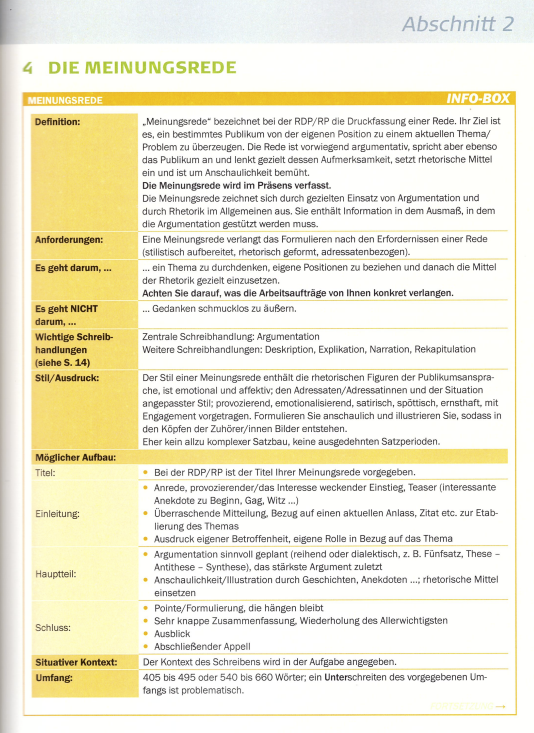
\includegraphics[scale=0.8]{pics/Screenshot from 2023-02-06 12-29-34.png}
    \caption{Meinungsrede: Definition + Aufbau}
    \label{fig:impl:Meinungsrede1}
\end{figure}

\begin{figure}[h][p]
    \centering
    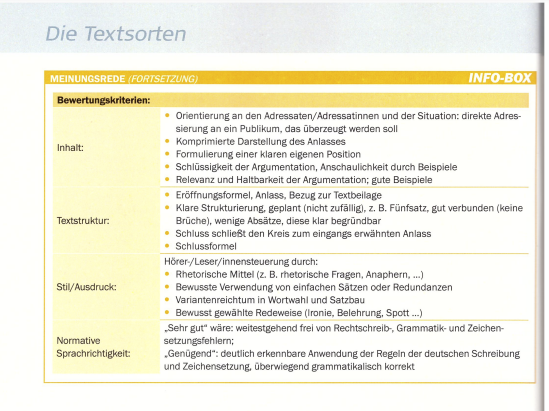
\includegraphics[scale=0.8]{pics/Screenshot from 2023-02-06 12-30-22.png}
    \caption{Meinungsrede: Verfassen}
    \label{fig:impl:Meinungsrede2}
\end{figure}
\begin{figure}[h][p]
    \centering
    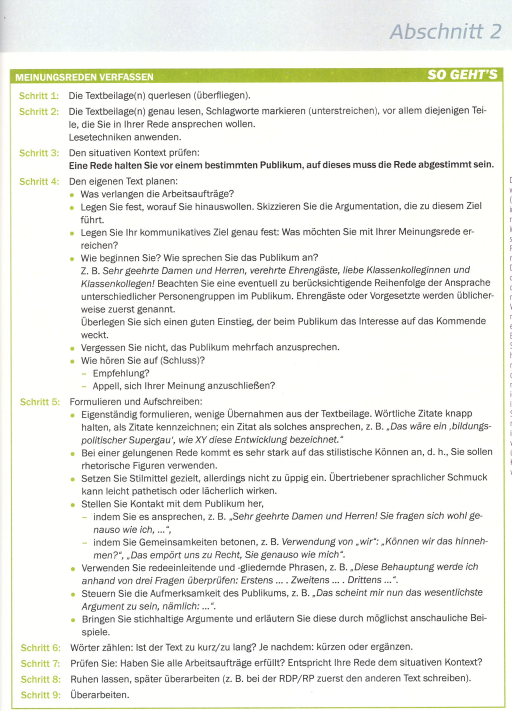
\includegraphics[scale=0.8]{pics/Screenshot from 2023-02-06 12-30-34.png}
    \caption{Meinungsrede: Fortsetzung}
    \label{fig:impl:Meinungsrede3}
\end{figure}

\section{Mustertext}
\subsubsection{Meinungsrede Zivilcourage}
Du blödes Kameradenschwein! Diese Aussage ist an niemanden im Publikum gerichtet, sondern fällt häufig im Umfeld von Menschen, die Zivilcourage beweisen. Doch, was ist das eigentlich, Zivilcourage? Viele kennen diesen Begriff nur aus Appellen von Politikern und Kirchenvertretern. Doch obwohl sie so wichtig ist und von so vielen gepredigt wird, ist sie fast nicht mehr in unserer Gesellschaft aufzufinden.  

Ich möchte zuallererst einen Fall aus den 60ern in den USA, genauer gesagt in Queens, neu aufrollen. Das Opfer ist Catherine „Kitty“ Genovese, eine Junge Frau, die eines Nachts mitten auf den Straßen New Yorks erstochen wird. Tja, spöttisch könnte man nun sagen, in den USA kann alles möglich werden. Der Täter war Winston Moseley. Dieses unmenschliche Monster hat nicht nur die Frau auf offener Straße, umringt von aufwachenden Anwohnern mit einem Jagdmesser erstochen, nein. Er kam später zurück, und stach erneut zu. Um seine Grausamkeiten noch abzurunden, vergewaltigte er die leblosen Überreste der armen Frau. Bitte bedenken Sie, dass dies immer noch mitten auf offener Straße geschah! In der Zwischenzeit hat niemand der dort Wohnenden seinen Allerwertesten hochbekommen, oder die Polizei verständigt. Und da soll man sich noch auf die Straße trauen? Muss man immer davon ausgehen, dass man von niemandem Hilfe bekommen wird? Leidet die Gesellschaft unter dem „bystander effect“? 

Dieser besagt nämlich, dass wir zu Herdentieren geworden sind. „Also, wenn die andern nichts machen, dann mach ich auch nichts“ – oder ähnliche Aussagen kommen dabei heraus. Die Menschen fürchten sich davor, sich zu blamieren und gehen davon aus, irgendjemand wird schon aufstehen und handeln. Verwunderlich, da wir doch alle die Superhelden aus Film und Fernsehen verehren und gerne wären wie sie. Die zeigen nämlich noch wirklich, was Zivilcourage ist, und dazu müssen sie nicht mal die Welt retten. Es reicht schon, wenn sie eine unschuldige Zivilistin retten. Der bystander effect ist der Bösewicht in unserem Blockbuster, und er ist nicht alleine. An seiner Seite kämpfen auch noch das Verlangen nach Harmonie, sowie der Drang nach Komfort. Sieht nicht gut aus für unseren Superhelden. Ob das ein Happy End wird? 

Fakt ist doch, wir wollen alle komfortabel leben. Und ein Außenseiter will man schon in der Volksschule nicht sein. Also immer schön mit dem Strom schwimmen, ja nicht anders sein und auffallen. Tarnkappenmodus aktiveren und unter dem Radar fliegen. Kurz gesagt: keiner will aus der Masse herausstechen. Es gilt als merkwürdig, und für manche auch als abstoßend, wenn jemand anders als der Rest ist. Doch genau hier sehe ich den Fehler. Es ist das „Mindset“, die Einstellung, die uns allen eingeprägt wird. Genau diese Barriere haben wir alle in unserem Gehirn. Nur die, die sie überwinden, können den anderen ein Vorbild sein. Doch um dieses annehmen zu können, müssen wir alle uns dazu bewegen, dieses Hindernis zu überwinden, zumindest es zu versuchen. Wir können nicht die Gesellschaft verändern, doch das muss auch nicht sein. Wir können und müssen uns selbst verändern, nur so kann die Meinung der Herde langsam gedreht werden.  

Um diesem Vortrag einen guten Ausklang zu verleihen, möchte ich Sie alle etwas bitten: Schauen sie nicht weg.  
Auch wenn es unangenehm ist: Schauen Sie nicht weg.  
Auch wenn es „schon jemand anders machen wird“: Schauen Sie nicht weg.  

Handeln Sie. 

535 Wörter 

\section{Eigener Text}
(Text aus dem Unterricht)
\subsubsection{Warum Sozialmedia nicht immer nur unterhaltsam und lustig ist. }

Wissen Sie, wer alles ihren Kindern heimlich über Social-Media Textnachrichten sendet? Theoretisch könnte es jeder sein. Ihr Nachbar, Ihre Schwester, selbst ihre Katze könnte anonym verstörende Nachrichten an die Kleinen versenden. Denkt denn keiner an die Kinder? Wie viele Bedrohungen und Beleidigungen die Kleinen wohl schon ertragen mussten? Wissen Sie, welchen Effekt unzensiertes Nutzen des Internets auf sich hat? Sehr geehrte Eltern, wann haben Sie das letzte Mal wirklich über die Gefühle Ihrer Kinder gesprochen? Heute geht es darum, wie Sie sich und vor allem ihre Kinder von äußerem Einfluss über die sozialen Medien schützen können. Denkt doch einmal an die Kinder. 

 

Es ist wie mit dem Masturbieren. Jeder tut es, keiner redet darüber. Wer von euch – und jetzt bitte ehrlich sein, – wer von euch war noch nie auf einem sozialen Netzwerk? Hat sich noch nie ein Video auf Youtube angesehen oder einen Post auf Facebook geliket? Jeder von uns, ja, wirklich jeder weiß, wovon ich spreche. Soziale Medien verändern unseren Alltag, verändern unsere Denkweise. Aber denkt wirklich keiner hier an die Kinder? An diejenigen, die ihre ganze Entwicklung noch vor sich haben, an die, bei denen der Einfluss von außen am meisten fruchtet? Keiner redet davon, wie sehr große Influencer auf TikTok oder Instagram die Jugend manipuliert. Für ihre Zwecke einsetzt. Welche Zwecke werden Sie sich jetzt fragen.  

Ganz einfach. Geld verdienen. Die Placements so gestalten, dass sie vor allem die junge Generation in die Irre führt und sie zum Kauf sinnlos teurem March bewegt. Auch die Denkweise, die freie Meinung und vieles andere kann von so bekannten Leuten schnell verändert werden. Und egal ob bewusst oder unbewusst, Menschen mit einer großen Reichweite haben eine sehr große Macht. Damals im Nationalsozialismus war es am Anfang nicht viel anders. Jeder schwimmt mit dem Strom, und der Rest hat Angst, darin unterzugehen, wenn er sich in die andere Richtung bewegt. Denkt doch einmal an die Kinder! 

Corona, die Ukraine, Russland oder die USA. Jeder bekommt immer die neusten Bilder, sieht grausame Videos aus Kriegsgebieten oder macht sich selbst zu einem Virologen. Soziale Medien haben unsere Art zu denken und Informationen auszutauschen, komplett verändert. Jedoch bekommen schon die Kleinsten von uns alles mit, – da sehr viele Wissenskanäle und Nachrichtenchannels auch online ihre Nachrichten ausstrahlen. Und da – wie jeder weiß, vor allem schlechte Nachrichten sich wie warmes Brot verkaufen, kann man auch hier wieder nur sagen: Denkt denn wirklich keiner mehr an die Kinder? An unsere Zukunft? 

Glauben Sie denn, es ist vorteilhaft, wenn die Kleinen von Anbeginn ihres Lebens mit schlechten Nachrichten konfrontiert werden? Wenn sie immer nur negative Sachen hören, gewalttätige Videos sehen oder in den Fokus von irgendwelchen Spaßvögeln geraten, welche sich daran aufgeilen, Menschen mit Drohungen Angst zu machen? Außerdem ist es als Elternteil sehr schwer zu kontrollieren, ob nicht irgendwelche pädophilen Menschen mit den Kleinen schreiben. Die sind dann meist noch so jung, dass sie nicht mal wissen, in welcher Gefahr sie sich befinden. Denkt doch einmal an die Kinder und schützt sie vor dem Einfluss von sozialen Medien 

 

Der letzte Punkt ist ganz kurz zusammengefasst: Mobbing. Über soziale Medien ist es schon fast Pflicht geworden, einen zweiten Account zu erstellen, mit dem man nicht in Verbindung gebracht werden kann. Und mit dieser Anonymität ist es dann ein Leichtes, einem Freund “Du H*rensohn” in die Kommentare zu schreiben. Der User wird sich nur denken, hach, das war lustig, während sein Freund vielleicht schwer von der Beleidigung getroffen ist. Auch hier denkt keiner an die Kinder. An diejenigen, bei denen Mobbing besonders groß und verbreitet ist. An diejenigen, welche durch Beleidigungen den größten Schaden anrichten. Auch hier kann ich nur an die Eltern appellieren: schränken sie den Gebrauch von sozialen Medien ein. Den Ihrer Kinder, aber auch Ihren eigenen. Soziale Medien können so viel Leid verursachen, und das alles nur, weil ein paar gute Programmierer mit der größten Schwäche des Menschen gespielt haben. Sie wollen Anerkennung. (Und vielleicht ein bisschen Geld muhahaha) 

\newpage

\section{Formulierungshilfen}
\subsubsection{Die Einleitung}
\begin{compactitem}
    \item … soll lebendig formuliert sein, da sie der erste Eindruck Ihres Textes ist und zum Weiterlesen / Zuhören animieren soll. Ein Trick der Rhetorik ist es, dass man Aufmerksamkeit durch Lachen oder Verstörung (= Provokation) erweckt. 
    \item  … soll das Thema beinhalten und erklären, warum Sie zu diesem Problem eine Rede halten. 
    \item    … ist von der Themenstellung abhängig. 
    \item  ... eindeutig den Redeanlass wiedergibt - hier sollte schon klar sein, welche Meinung Sie vertreten.  
\end{compactitem}
\subsubsection{Der Hauptteil}
\begin{compactitem}
    \item … ist der längste und ausführlichste Teil Ihrer Rede. 
    \item … enthält nur Argumente, die Ihre Meinung untermauern. Ein Trick der Rhetorik ist es, dass Gegenargumente angesprochen werden, aber als nichtig abgetan werden, um der eventuellen Gegenkandidatin / dem eventuellen Gegenkandidaten den Wind aus den Segeln zu nehmen. [Beispiel: Hier könnten wir natürlich auch … ins Treffen führen, aber das führt zu nichts, weswegen ich hier nicht näher darauf eingehen möchte.] 
    \item … soll auf das Auditorium Bezug nehmen und in diesem Teil wird es auch immer wieder gezielt angesprochen. Achtung! Sie müssen die Situierung genau lesen, denn wenn Sie als Schüler/in/ Ihre Schulkolleg/innen ansprechen, dann werden Sie diese sicherlich nicht Siezen. Andererseits würden Sie die Direktorin / den Direktor oder Vorgesetze wahrscheinlich nicht duzen. 
    \item … soll rhetorische Mittel enthalten, um die Argumentation zu unter-stützen. [Anm.: Sie sollten sich hier nicht unnötig in Panik versetzen, da wir generell in Figuren sprechen. Es gibt 160 000 verschiedene Stilmittel, aber Sie werden höchstwahrscheinlich mit den gängigsten punkten können. 
\end{compactitem}
\subsubsection{Im Schlussteil}
\begin{compactitem}
    \item  … soll das Wesentliche kurz zusammengefasst werden. 
    \item    … soll ein Appell oder gar ein Lösungsvorschlag an das Publikum ge-richtet werden. Das entnehmen Sie aber den Arbeitsaufträgen! Beachten Sie hier, dass Sie unbedingt das Verbum "appellieren" verwenden! Beachten Sie die Zielgruppe - an wen wendet sich meine Rede?
\end{compactitem}

\subsection{Realitätsbezug}
Die Rede kommt vor allem in der Politik vor, und ist ein sehr wichtiger Bestandteil, um eine große Anzahl der Menschen für sich zu entscheiden.  

\subsubsection{Beispiele für verwandte Textsorten}Gelegenheitsrede, Überzeugungsrede, Feierrede, Ansprache, politische Rede, Aufruf
\subsubsection{Abgrenzung} Die Meinungsrede zeichnet sich durch ihren gezielten Einsatz von
Argumentation und Rhetorik im Allgemeinen aus. Sie ist dabei nicht
zwingend politisch oder an einem politischen Anlass orientiert, wie
etwa die politische Rede. Die eigene Position steht bei der Meinungsrede im Vordergrund, sie wird jedoch untermauert und das Publikum
miteinbezogen. Sie informiert und erklärt nur so weit, wie notwendig,
um die Argumentation zu stützen.
\subsubsection{Umfang} 405 bis 495 oder 540 bis 660 Wörter
\subsubsection{situativer Kontext} erforderlich
